% \documentclass[12pt,english]{article}
% \usepackage[affil-it]{authblk}
% \usepackage{graphicx}
% \usepackage[space]{grffile}
% \usepackage{latexsym}
% \usepackage{textcomp}
% \usepackage{longtable}
% \usepackage{multirow,booktabs}
% \usepackage{amsfonts,amsmath,amssymb}
% \usepackage{url}
% \usepackage{hyperref}
% \hypersetup{colorlinks=false,pdfborder={0 0 0}}
% %\usepackage{latexml}


\documentclass[12pt,english]{article}
\usepackage[utf8x]{inputenc}
\usepackage{graphicx,latexsym,longtable,multirow,booktabs,amsfonts,amsmath,amssymb,url}
\usepackage{rotating,subcaption,marginnote}


\usepackage{natbib}
\setcitestyle{round}

\usepackage[colorinlistoftodos]{todonotes}
\usepackage{comment}

\begin{document}

\title{An Evaluation of Option Contracts in Semiconductor Supply Chains}




\author{Cathal Heavey}
%\affil{Affiliation not available}



\date{\today}



\maketitle 

\listoftodos




\begin{comment}
\begin{enumerate}
\item I feel you need to write this paper as a chapter, then take from this chapter a paper. This will reduce the risk to you as you will not have to wait for replies from journals. It will also, hopefully, make it easier to write a journal paper from a chapter.
\item You could bring in results and sections from the earlier paper into this chapter or paper. 
\item In developing the options model you need to present a rationale for it using the referenced citations that you have in the paper and possibly other references as well. This is important for me.   
\item Forecast error with variance of 40 and in section 4.2 $\sigma=20$. ??
\item Need to use standard terms throughout the paper. 
\item You need to explain everything in the paper, for example, you use "DP Volume Weighted" in Figure 2, with no explanation given.
\item You need to explain all results, for example, on page 17 you state that $DP$ reduces as $o$ increases.
Why is this the case? For example, are you calculating $DP$ correctly? Is there an error in your model?
\item There is no verification or validation of your model within this paper. This is a very important issue -- two do we know that the model developed is valid? Note, the first model was validated in the earlier paper published, which you cam reference. Here emphasis must be given to validating and verifying the options model, as this model is newly introduce in this chapter/paper. Is it possible to validate verify the option results with other models? Probably not?
\item There are mistakes in the paper, which I note.
\item The results of the experimentation does not make much sense, where you comparison on one result from the RHF paper and show other results from the options paper where you try to optimize $o$. These results need to be deeply reviewed.
\item There are no costs in the model, how will someone interpret Table 3? 
\end{enumerate}
\end{comment}



\begin{abstract}% Need to check
This paper considers a supply chain that comprises of three parties:
a customer, a supplier (semiconductor manufacturer), and a capacity 
provider in which two different contracts are compared:
a quantity flexibility contract and an option contract. Informed by the
characteristics of actual clauses and demand behaviours drawn from
a company's experience, a discrete-event simulation model is developed
to represent the company's supply chain. Under a quantity flexibility
contract, the customer forecasts a quantity of units and has the
right to modify his forecast within the rolling horizon quantity flexibility
clauses before passing his final demand. In an option contract the
customer pays an upfront fee (option price) for an option
to buy a product, which gives the customer the right but not the obligation
to execute and therefore buy the product within a certain delivery
window. To exercise the option, the customer has to pay the exercise
fee. In case customers final demand exceeds the bought amount
of options, the customer can buy additional supply on the spot market
for a spot price. Within both contracts, the customers
forecast is subject to error. Firstly, the theoretical bases are introduced
for each contract type, next both models are compared. Simulation
is used to compare the performance of an option contract against a
capacity reservation contract with order flexibility clauses used
in a semiconductor supply chain in terms of delivery performance and
overall supply chain profit. The simulation results are presented
and discussed followed by the conclusion. This is a test New test% Need to insert details of the results
\end{abstract}%


\section{Introduction}

This work compares the supply chain performance under a capacity reservation
contract with order flexibility clauses typically found in the semiconductor
industry and an option contract. Extreme variability in capacity utilization
is an established characteristic of the semiconductor industry. Important
factors in this volatility are, at one level economic cycles leading
to amplified fluctuations in end product demand, at another the incessant
progress in innovation and consequent shortening of product life cycles
to the degree that they are measured in months.  
Consequently, semiconductor
manufacturing customers request and expect high levels of order flexibility
and short order lead-times to align with changing market demands and
contexts. This creates major challenges for semiconductor manufacturers
due to substantially longer physical production cycle times when compared
to the requested order lead times. Sharing of forecast information
between customer and semiconductor manufacturer is necessary in this
industry, but it alone is not sufficient to manage effectively this
demand volatility. Game-playing is common: customers inflate their
demand forecasts to ensure the semiconductor manufacturer builds enough
capacity, while the manufacturer plans conservatively to avoid overcapacity
and to stay cost competitive. This behavior can result in tight supply
and allocation difficulties for the manufacturer, and also downtime
and lost revenue for customers. The use of options in supply chains
is gaining increased attention: the customer pays an upfront fee (option
price $p_{o}$) for an option to purchase a product, which gives the
customer the right but not the obligation to execute and therefore
buy the product for the exercise fee $p_{e}$. The option price is
an upfront payment by the customer to the manufacturer for building
and reserving the respective products. The exercise fee is the payment
by the customer to the manufacturer for excising one unit of the option.
In addition to the option contract, the customer can purchase supply
on the spot market for the  price $p_{s}$, with product not exercised  by the customer being placed in the spot market. In the literature,
spot markets have not often been included in supply chain contract
models.  %% Konstanze can you add a cite here as you stated "not often" which means that this has been cited %. 
Spot markets are used by manufacturers to clear excess production and by customers
to to buy additional supply in case of shortages. Option contracts
are claimed in the literature to enhance supply chain flexibility
through exercising the right to change order quantities.% Please cite there here, you cannot make this claim and not cite  
Upfront payments
compensate supply-side manufacturers for costs where a customer does
not exercise its option to buy. Options are generally tied to a contract
and cannot be traded between supply chain members. This kind of option
is called \textquotedblleft nested option\textquotedblright{} \citep{Wang2011a}.
We consider the situation of one customer and one supplier under demand
uncertainty and compare the results for the chain of two cases: when
a capacity reservation contract with order flexibility is set in place
and when an Option Contract is used under three different customer
demand behaviors (No bias, under planning, over planning). This paper
is organized as follows. Firstly
we present the literature review of contracts with order flexibility
and Option Contracts. Then the forecast and ordering process found
in the case study is presented followed by the analysis of the customer
order behavior. Next, the model is presented. Then the model is simulated
for different scenarios and the results of the simulation are discussed
followed by the conclusion. 

\section{Literature Review}

\paragraph{Contracts with order flexibility}

Donohue (2000) models a manufacturer\textquoteright s supply-side
flexibility in a two-stage supply chain by giving the supplier two
production modes, normal and fast. The fast mode allows the customer
to order additional parts to take advantage of updated demand forecasts.
The objective is efficient conditions for channel coordination. The
performance measure is total profit. \citet{Walsh2008} simulated
two types of contracts between an original equipment manufacturer
(OEM) and a contract manufacturer (CM) in a supply chain: one with
constant flexibility boundaries and the other with decreasing flexibility
boundaries. They stated that measured by fill rate, bullwhip effect
and inventory level both contracts have for OEM and CM favorable results.
Regarding the design parameters of the quantity flexibility contract,
the upper and the lower bound rates of the flexibility profile were
assumed stationary and symmetric as also in the work of \citet{BassokAnupindi2008}.

The latter work analyzed an open loop feedback control based heuristic
algorithm for the contract and demonstrated numerically that with
decreasing flexibility, the order process variability decreases significantly.
They also provide insights on how much flexibility is sufficient from
a buyers perspective and its effect on customer satisfaction.

\citet{Wang2008} investigated the advantages of a supply chain with
different degrees of order quantity and delivery lead time flexibility
and derived that lead time flexibility allows the buyer to improve
its service level and reduce the shortage cost, when the cost per
shortage is relatively high. Furthermore the author noted that service
level should be maintained at least at a certain level to keep customers\textquoteright{}
loyalty.

\citet{Kim2011} analyzed a quantity flexibility contract between
a buyer and a supplier and showed the supplier\textquoteright s trade-off
between the customer service level and the inventory risk. Whereas
for the buyer, the benefit keeps increasing and then remains constant
as the flexibility rate increases. In general the author stated that
in a decentralized system, the quantity flexibility contract can provide
an effective coordination mechanism for the supply chain.

As in \citet{Kim2011}, this work will consider both, the supplier\textquoteright s
as well as the customer\textquoteright s view by analyzing the impact
of contract individually and on the overall supply chain. The focus
of this work is on the order flexibility in terms of quantity and
order lead time. This work is not intended to derive optimal ordering
and inventory policies given an implementation of the contract as
the optimal policies associated with quantity flexibility would be
extremely complex and unattractive for implementation \citep{BassokAnupindi2008}.

\paragraph{Option contracts }

\citet{Cachon:Lariviere2001} model flexibility through options in
a two-stage buyer-supplier contract where the buyer makes a firm commitment
and buys additional options with the supplier installing capacity
accordingly. After demand is realized, the buyer has the right to
exercise their options. The contract is studied under forced and voluntary
compliance regimes and the performance is measured for individual
supply chain participants and the whole supply chain. \citet{Cheng2003}
presented a variant of an Option Contract focuses on the optimal order
decision of the buyer and the optimal pricing decision of the supplier.
\citet{Barnes-Schuster2002b} use options to find a better order distribution
along the periods of contract validity in a two-stage two-period supply
chain under correlated demand. Again, the customer initially places
firm orders for two periods and buys additional options; after observing
demand in the first period, the buyer can increase from their initial
demand quantity for the second period by exercising their options.
Their performance focus is cost: before and during the first period,
the supplier produces at a regular cost, and from the beginning of
the second period but after the options are exercised, the supplier
produces at an extra cost. Options are shown to improve channel performance,
and an appropriate price for channel coordination is derived. \citet{VanDelft2004}
provide an extended implementation of this model using stochastic
programming including numerical performance estimation from various
contractual parameters like costs and revenue. \citet{M.Erkoc2005}
model capacity reservation contracts with deductible reservation fees
and exogenous wholesale prices: the customer buys capacity reservations
and pays the reservation fee offered by the supplier who then decides
how much capacity to build. After demand uncertainty is resolved in
time, the customer exercises all or part of the reserved capacity.
Within this context, the authors investigate individual rationality
and channel coordination. They also consider different compliance
regimes and partial information updates. The supply chain profit is
a function of the wholesale price the supplier\textquoteright s production
costs and the capacity level. The authors stated that the supply chain
profit of a capacity reservation contract with a fully deductible
reservation fee is suboptimal unless the customer\textquoteright s
reservation quantity is equal to the supplier\textquoteright s capacity.
In a single-period, two-stage supply chain, \citet{Wang2006} introduce
a bidirectional Option Contract: the buyer has the possibility to
adjust the initial order both downwards and upwards. If the buyer
exercises his options as call options, then he pays a unit exercise
price for each exercised option whereas he can get back a corresponding
full or partial refund if he exercises the options as put options.
Outcomes were evaluated from the buyers\textquoteright{} perspective
and optimal policies were developed for the buyer. A uniformly distributed
stochastic demand was used. \citet{Wang2007} develop an option-based
contract model to study channel coordination and risk sharing in a
decentralized retailer-led supply chain: the Option Contract has an
option price and exercise price, and the retailer has to pay the option
price for each unit reserved above the initial order quantity, and
for each called option the retailer has to pay the exercise price.
They found that two conditions are necessary for a successful coordination:
firstly to maintain a negative correlation between exercise price
and option price, and secondly that the firm commitment must be lower
than the optimal production quantity of a corresponding centralized
system. Under these conditions they conclude that the option-based
contract model performs better in terms of profit than the traditional
price-only contract model. \citet{Gomez-Padilla2009} study an Option
Contract in a two-stage retail supply chain with one retailer and
either one or multiple suppliers. The suppliers and retailer\textquoteright s
benefits are measured by their own revenues diminished by their individual
costs. The authors showed that an Option Contract in a supply chain
consists of one retailer and one supplier will increase the benefit
for all supply chain partners as well as for the chain. Variation
in demand is modeled as exogenous. Similar to approach from \citet{Gomez-Padilla2009},
\citet{M.Erkoc2005} compared partial payment deduction and reservation
with cost sharing, where the partial payment deduction corresponds
to the deductible reservation in \citet{Gomez-Padilla2009} and the
reservation with cost sharing corresponds to a setting where the supply
chain partner share the cost of the capacity reservation and where
the customer either receive a refund or has to make a additional payment
after final demand is realized. Both papers, \citet{Gomez-Padilla2009}
and \citet{M.Erkoc2005} analyzed capacity reservations in the context
of high-tech industries. \citet{BassokAndAnupindi1997} analyzed a
model for an Option Contract where the customer orders a fixed quantity
at each period and additionally a number of units as options for demand
the customer may require. To put these options, the customer has to
pay a fixed price and an additional price in case options are exercised.
The authors modeled a normal distributed and correlated demand and
determined the number of options to reserve in order to maximize the
profit. \citet{Zhao2013375} analyzed a bidirectional Option Contract
for a supply chain consistent of a manufacturer and a retailer. The
authors derived closed-form expressions for the retailers optimal
order strategies under a general demand distribution. They showed
that there are fundamental differences between the single directional
option and the bidirectional Option Contract. \citet{Gomez-Padilla2009}
compared the performance of an Option Contract with a wholesale price
and a buy-back contract in a multi period setting. They used simulation
to demonstrate that an Option Contract can benefit each supply chain
partner as well as the overall supply chain. \citet{Gomez2013} compared
a capacity reservation contract with an Option Contract in a two echelon
supply chain under uniform demand and uniform increasing demand. They
concluded that an Option Contract provides higher benefits to the
retailer, but a capacity reservation contract will benefit the supplier
and the whole supply chain. Our paper is most related to the literature
which focuses on bidirectional adjustments over the initial order
within a two echelon supply chain. The customer determines the orders
for the upcoming periods, at the beginning of the planning horizon.
Within the final demand, the customer is able to adjust the amount
of options he wants to exercise accordingly. In case the customer
needs a higher quantity than initially reserved as options, the customer
is able to source it at the spot market. 

While in the presented work above the customer demand signal was modeled
as a stochastic process without any bias, in this work the demand
signal is subject to forecast error which is explicitly modeled with
an over or under planning bias. Furthermore, the forecast variability
is changing over the forecasted horizon, which means that the forecast
error decrease with approaching delivery date, in order to simulate
realistic customer demand behaviors as found in the case study company.
As the variability of the forecast error is not symmetric, we will
also investigate non symmetric upper and lower flexibility boundaries.

\section{Model Description}

This work is based on a research project at one of European biggest
semiconductor manufacturer from January 2010 to October 2013. Within
the case study, deep knowledge about the manufacturers internal processes,
the customer order behavior and contract clauses was developed. The
Supply Chain contracts at the case study company defining the different
agreements with its customers; either with direct customers or with
distributors. The main SC contracts that was currently set in place
with its direct customers are the basic supply agreement, the consignment
agreement, the capacity reservation agreement and the reduced lead
time agreement (Knoblich, 2013). More than 250 contracts were collected,
reviewed and analyzed within the project. These different contracts
represent the rules that both partners have to comply with when they
are planning their supply chain operations. Furthermore, Customer
forecasted accuracy reporting was investigated. Based on this knowledge,
the simulation model was build. Real customer forecast data and analysis
where used to evaluate the right parameters for the simulation model.
All parameters, which were set within the demand signal generator
where derived from companies forecast accuracy measurement reporting.
This reporting compares the customer forecasts with the actual customer
billings. Within this reporting, parameters of the demand signal generator
could be set in a manner to simulate the same heaviness of order volatility
as in the real live.

The supply chain model considered in this study is a two echelon supply
chain, consisting of a customer and a semiconductor manufacturer involving
a perishable product, which has a comparatively long production lead
time and short order lead time. In this study a representative capacity
reservation contract with order flexibility (RHF Contract) found in
the semiconductor sector is compared with an Option Contract. The
objective is to compare these contracts under different customer demand
behaviors. The analysis in the contract market is limited to one supplier
and one customer. However, competition by other suppliers is included
indirectly via the demand function. The extension of the model to
multiple customers is straightforward: The current single customer
can be interpreted as the aggregation of all customers. Initial demand,
$D_{i}$, is assumed stochastic and there are no back orders. The
cancellation clauses is not explicitly modeled as it can be seen as
an extension of the downside flexibility. The supplier is assumed
to have unlimited capacity, through internal and outsourced facilities,
but capacity has a fixed lead time $Lc$. Within this lead time the
supplier\textquoteright s capacity is fixed. In practice $L_{C}$
is in the range of 8-12 months.

\subsection{Customer Demand}

The customer\textquoteright s forecast is an expected value $D(t)$
for time $t$ calculated from the actual demand at the previous period
of time $D(t-1)$, subject to a forecast error $r$. This is shown
in the figure \ref{fig:Customer-Demand}. We assume that the manufacturer
tries always to satisfy the customers demand in full. The initial
demand is modeled using a gamma distribution. The standard gamma is
a continuous distribution with two parameters that provide good control
of the shape of the distribution. The reasons for choosing this distribution
are that it is positively skewed and allows high values of coefficient
of variation. The density function of the gamma distribution is generated
according to the following formula:

\begin{equation}
\frac{\beta^{-\alpha}x^{\alpha-1}e^{-\frac{j}{\beta}}}{\Gamma(\alpha)}\label{eq:equation4}
\end{equation}


with the mean$\mu$ and the variance $\sigma$ of the $G$ distribution
given by $\mu=\alpha\beta$ and $\sigma^{2}=\alpha\beta^{2}$ with
the shape parameter $\alpha$ and the inverse scale parameter $\beta$
. The forecast error is modeled using a normal distribution 
\begin{equation}
D_{j-1}\sim\mathcal{N}\left(\left(D_{j}+\mu_{f}\right),\sigma_{j}^{2}\right),\quad j=52,t-1,\cdots0\label{eq:normal}
\end{equation}
Furthermore, the variance of the forecast error decreases with the
decreasing time difference ($\Delta t$) between the period of time
$t$ in which the forecast is generated and the requested delivery
period of time $j$. Let 


\begin{equation}
\sigma_{j}=\sigma_{f}+m\times\Delta t\quad\triangle t{\textstyle \;{\textstyle \textrm{and}}}\; j=52,51,\cdots,0\label{eq:Variance}
\end{equation}
where $\sigma_{f}$ equals the fitted forecast error for a customer
and $m=1$ in this case. A mean of $\mu_{f}=0$ is used to model an
unbiased customer or a shifted normal ($\mu_{f}\neq0$) for a customer
that over or under forecasts. These relationships allow modeling of
a forecast accuracy error which gets smaller as the delivery date
approaches, which was observed in the case study company. 

\begin{figure}[h!]
\begin{center}
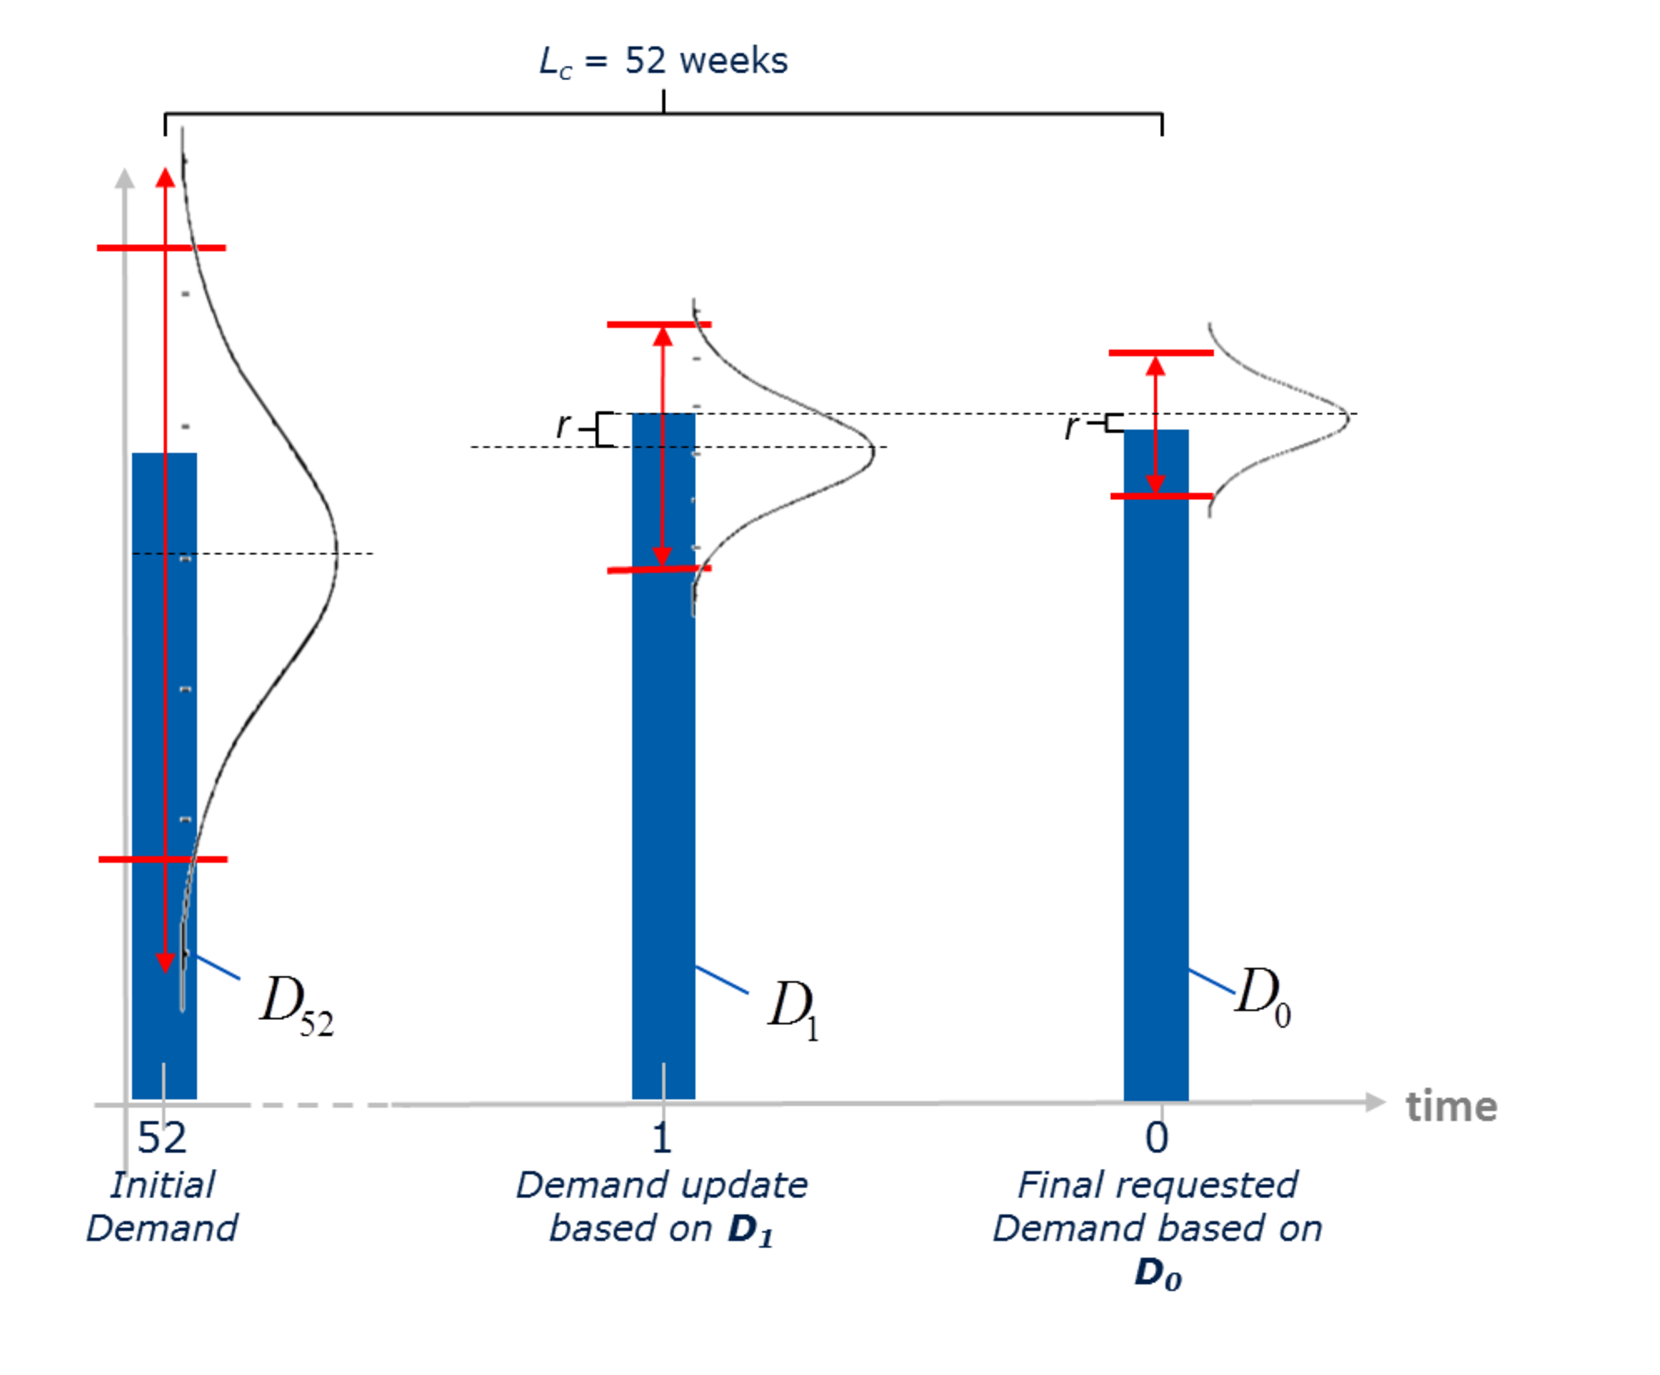
\includegraphics[width=0.7\textwidth]{Figures/Demand_Generator.eps}
\caption{Customer Demand}%
\label{fig:Customer-Demand}
\end{center}
\end{figure}




\subsection{Capacity Reservation Contract}

Within the capacity reservation contract with order flexibility are
two operational clauses that govern the contract: (i) the order lead
time that governs the time within the customer has to place his order
prior to the requested delivery date of the order, which the supplier
use to finalize last production steps and to deliver the products
(ii) quantity flexibility that governs the changes in the quantity
of the customer order. Temporal ordering of the operational sequences
in each time period is as following:

\begin{enumerate}
\item In the standard contract model, the customer provides his weekly rolling
demand forecast $D_{j}^{t}$ for period $j$ forecasted in period$t$,
$Lc$ periods before the first scheduled delivery. This forecast is
subject to a forecast error;
\item The semiconductor manufacturer will source capacity and produce supply
accordingly to the customer\textquoteright s demand forecast in order
to meet the monthly aggregated demand for period $Lc$;
\item The customer updates his demand on a weekly basis until $t=j$;
\item The semiconductor manufacturer evaluates the customers final Demand
$D_{j}^{t}$ according to the operational clauses and confirms demand
accordingly;
\end{enumerate}
The standard contract used in this paper consists of two supply chain
operational contract clauses. The quantity flexibility clause gives
the customer the right to change his initial demand forecast quantity
within the rolling horizon flexibility boundaries. The clause can
be expressed as follows:

\[
(1-\gamma_{tj}^{L})D_{j}^{t-1}\leq D_{j}^{t}\leq(1+\gamma_{tj}^{U})D_{j}^{t-1}whent\leq j
\]

\[
D_{t}^{t}=D_{t}otherwise
\]

where $D_{j}^{t}$ is the customers demanded quantity for period $j$
forecasted in period t. $y_{tj}^{L}$ and $y_{tj}^{U}$ are the lower
and upper flexibility bounds for period $j$ at period $t$. This
equation gives the customer the right to adjust his demand according
to his latest demand information until$t=j$. When$t=j$, the demand
is the final requested demand and is indicated as $D_{t}^{t}=D_{t}$
. The second clause relates to cancellation. Specifically, the customer
can cancel his forecasted demand by a percentage $p$ within a specified
time period, defined as $[i_{a}^{p},i_{b}^{p}]$ over $T$, where
$i_{a}^{p}$ , $i_{b}^{p}$ define the start and the end of the period
where $p$ percentage of an order can be canceled without penalty.
For the experiments presented in this paper, the parameters $p$ for
the cancellation clauses is set to 0. This is justified as the cancellation
clause only extends the lower flexibility boundary. The same effect
can be achieved by decreasing the lower flexibility boundary. All
customer orders which are below the lower boundary, can be viewed
as cancellations for which the customer has to pay a cancellation
fee of 100\% of the product price.

\begin{itemize}
\item $D_{j}^{t}:$Customer forecasted demand in time $t$ for time period
$j$
\item $D_{t}$: final customer demand in period $t$
\item $\gamma_{tj}^{L}$: lower flexibility bounds in period $t$ for time
period $j$
\item $\gamma_{tj}^{U}$: upper flexibility bounds in period $t$ for time
period $j$
\end{itemize}

\subsection{Option Contract}

In the second situation the customer orders a certain amount of options
for specific delivery windows $o$ and pays the option price $p_{o}$
upfront for each unit. Within the respective delivery window $o$,
the supplier gives the customer the liberty to exercise his options
for the execution fee $p_{e}$ as he wants. The customer has two order
sources, namely the contract market and the spot market. In case the
customers final demand exceed the bought amount of options, he can
source additional supply on the spot market for the spot price $p_{s}$.
The options contract operates as follows:

\begin{enumerate}
\item The customer forecasts demand $Lc$ periods before the delivery date.
This forecast is subject to a forecast error;
\item The customer purchases options based on this first initial forecast
for delivery window $o$; 
\item Based on these options the semiconductor manufacturer reserves production
capacity and produce the respective supply; 
\item The customer can exercise for the exercise fee $p_{e}$ his options
with full flexibility within the delivery window $o$; 
\item Supply which was not consumed by exercising option, will be made available
on the spot market; 
\item If the customer cannot satisfy demand through exercising his options,
product can be purchased from the spot market.
\end{enumerate}
In the Option Contract model, the customer decides how much options
$D(t)$ he wants to buy for the delivery window $o$, $L_{c}$ periods
before the first scheduled delivery in delivery window $o$. The supplier
will reserve capacity equal to the amount of options purchased in
order to meet aggregated demand for delivery window $o$. For each
option the customer has to pay the option price $p_{o}$ and for each
exercised option the exercise price $p_{e}$. If the customer does
not exercise all purchased options for a certain delivery window $o$,
the option price serves as a compensation fee for the customer who
will incur production cost for these options. The non exercised options
are transferred to the spot market. In the case where the customer\textquoteright s
demand exceeds his options, he can buy additional products on the
spot market for price $p_{s}$ assuming that the spot market has available
products. When $p_{e}=0$, $p_{o}$ can be seen as the \textquotedblleft wholesaler\textquotedblright{}
price and the contract between customer and supplier as a fixed commitment
contract. When $po=0$, which is the case for the standard contract,
the contract can be seen as wholesaler contract with a non binding
forecast. When $p_{e}>0$ and $p_{o}>0$ the contract can be thought
as an Option Contract with an option price of $p_{o}$ and an execution
price of $p_{e}$. In the experiments described in this paper the
option price is set at one third the standard product price ($p_{std}$)
where $p_{std}=p_{o}+p_{e}$. The spot price includes the standard
product price pstd plus the average price decline $p_{d}$ and average
inventory and price decline costs, $i$, per period $t$, with $p_{s}=p_{std}+p_{d}+i.$

\begin{itemize}
\item $o$: Delivery Window to exercise options
\item $p_{o}$: Option Price
\item $p_{e}$: Execution Fee
\item $p_{s}$: Spot Market Price
\item $i$: inventory and price decline costs
\item $p_{std}$: Standard Price
\end{itemize}

\subsection{Performance Metrics}

The performance measures used in the experimentation are the delivery
performance (DP), Billings (B) and the Inventory level (I). Delivery
Performance is calculated as the total number of products delivered
on time and in full based on a customer requested date (Supply Chain
Council, 2010; Vickery, Droge, \& Markland, 1997). DP is a demand
fulfillment measurement which compares the customers final requested
demand, with the quantity of delivered products (Billings), B. Let
the delivery performance Delivery Performance equal for a product
delivered to a customer be

$DP_{i}=\frac{B}{D_{o}}x100$

\[
SupplyChainProfit=Billings-(Costs_{Seller}+Costs_{Buyer})
\]

with for all products delivered to a customer during the simulation
model of length K in which results are collected. This measurement
can be seen as a performance index of customer satisfaction, i.e.
the customer final demand is 100 pieces, but the semiconductor manufacturer
is only delivering 90 pieces (B), then the DP would be 90\%. 
chain Profitability can be calculated by Revenue generated from a
customer minus the total cost incurred to produce and deliver the
product \citet{Sunil2012}



\section{Experimental Plan}

\subsection{Customer order behavior setting}

\textcolor{black}{The initial customer forecast demand $D_{i}$ for
the first 52 weeks is modeled by using a gamma distribution. Real
customer data from the case study company were analyzed and curve
fitting methods were applied, to derive realistic values for the gamma
distribution parameters. Based on the analysis of a representative
customer, a shape parameter $\alpha$ of 80 and the inverse scale
parameter $\beta$ of 20 was identified and used for the following
experiments. $D_{i}$ is updated on a rolling horizon principle and
is subject to forecast error which is modeled be using a normal distribution.
Real forecast error data of an unbiased customer order behavior were
analyzed and a forecast error variance of 40 was observed, one week
before final demand $D^{t}$. In order to model the three different
order behaviors unbiased, over planning and under planning, the mean
$\mu$of the normal distribution was set to 0, -20 and +20 which reflect
a common bias at the case study company.}

\textcolor{black}{The three different customer forecast accuracy settings
are summarized in Table}\textcolor{red}{{} \ref{tab:Customer-Demand-Signals}},
e.g.\textcolor{black}{{} The demand signal D2 represents a customer,
who has a tendency to under forecasting, i.e. $D_{j-1}^{t}<D_{j}^{t}$. }

\begin{table}
\centering{}\protect\caption{Demand values for forecast error distributions\label{tab:Customer-Demand-Signals}}
\textcolor{black}{}%
\begin{tabular}{|l|c|c|}
\hline 
\textcolor{black}{Initial Customer Demand Signal} & \textcolor{black}{$\alpha=80$} & \textcolor{black}{$\beta=20$}\tabularnewline
\hline 
\multicolumn{1}{l}{} & \multicolumn{1}{c}{} & \multicolumn{1}{c}{}\tabularnewline
\hline 
\textcolor{black}{Forecast error} & \textcolor{black}{$\sigma_{i}$} & \textcolor{black}{$\mu$}\tabularnewline
\hline 
\hline 
\textcolor{black}{D1 - no bias} & \textcolor{black}{40} & \textcolor{black}{0}\tabularnewline
\hline 
\textcolor{black}{D2 - over planning bias} & \textcolor{black}{40} & \textcolor{black}{-20}\tabularnewline
\hline 
\textcolor{black}{D3 - under planning bias} & \textcolor{black}{40} & \textcolor{black}{20}\tabularnewline
\hline 
\end{tabular}

\end{table}

\subsection{Option Contract settings}

For the options contract, different delivery window
lengths were considered across different customer order behavior:
unbiased, under planning and over planning. The simulated delivery
window lengths evaluated are $o={1,...,13}$. Forecast error is modeled
using the normal distribution, as described in the previous Section,
with $\sigma=20.$ Figure \ref{fig:Overview-of-Option} presents
results showing the performance of the Option Contract measured using
billings, B, delivery performance, DP, and Inventory, I. Results are
presented for customer demand behavior with no bias, with over planning
and under planning bias. First, in all cases DP decreases as o increases.
It is not obvious why this is the case, however, it could be the result
of the result of the greater granularity of option allocation with
lower values of o. Whereas the Billings stays almost stable or slightly
increase as o increase. This probable results form the fact that as
o increase the customer has greater flexibility, due to a larger delivery
window, i to exercise purchased options. The results also show that
the Billings are greater for the under planning behavior and Billings
are lower than for the no bias behavior. This is because a customer
that under forecasts will have more options to exercise than what
will be required. The over planning bias shows a higher DP then for
under planing bias, but also and decreasing trend within increasing
o.

\subsection{Evaluation of Option Contracts versus Capacity
Reservation Contract}

This section further evaluates an Option Contract
by comparing it with a standard contract typically used in semiconductor
supply chains. The performance of the standard contract with a RHF
clause is highly dependent on the upper and lower flexibility bounds
($y_{jt}^{U},y_{jt}^{L}$) used (Walsh, Williams, and Heavey 2008).
According to a previous work (Knoblich et al. 2015) unsymmetrical
flexibility bounds show a higher performance than symmetrical flexibility
bounds for over and under planning customer order behavior. Therefore
we simulated 36 different flexibility settings for each demand signal
(D1 - D3) to establish the most appropriate values
for ($y_{jt}^{U}$ , $y_{jt}^{L}$) for a fair comparison of the standard
contract with the Option Contract. Starting from zero flexibility,
the upper and lower flexibility bounds were increased incrementally
by 0,1. The simulated upside and downside flexibility rates are shown
in Table \ref{tab:Upside-and-Downside-1} In comparing
the contracts, standard and option, both were simulated with the same
demand signal parameters, which are $\alpha=80$ and $\beta=20$ for
the gamma distribution and a sigma of 20 for the normal distribution
in order to generate the forecast error. A neutral forecast error
$\mu=0$ was used for a biased customer order bahavoir and $\mu=-20$
for over planning and $\mu=20$for under planning behavior. For the
Option Contract, different delivery window $o=\left\{ 1,..,12\right\} $
lengths were considered. 

\begin{table}
\begin{tabular}{|c|c|c|c|c|c|}
\hline 
Contract Settings &  & \multicolumn{4}{c|}{Starting Point of upside Flexibility}\tabularnewline
\hline 
 &  & \multicolumn{1}{c||}{\textbf{0}} & \multicolumn{1}{c||}{\textbf{0.1}} & \multicolumn{1}{c||}{\textbf{0.2}} & \textbf{0.3}\tabularnewline
 \hline 
 \multirow{4}{*}{Starting Point of downside Flexibility} & \textbf{0} & A1 & A2 & A3 & A4\tabularnewline
 \cline{2-6} 
  & \textbf{0.1} & B1 & B2 & B3 & B4\tabularnewline
 \cline{2-6} 
  & \textbf{0.2} & C1 & C2 & C3 & C4\tabularnewline
 \cline{2-6} 
  & \textbf{0.3} & D1 & D2 & D3 & D4\tabularnewline
 \hline 
 \end{tabular}

% Reading Example of Table:%
\begin{tabular}{|c|c|c|c|c|}
\hline 
\multirow{2}{*}{A1} & upside flexibility & 0 & 0.1 & 0.2\tabularnewline
 \cline{2-5} 
  & downside flexibility & 0 & 0.1 & 0.2\tabularnewline
 \hline 
 \end{tabular}%
 \begin{tabular}{|c|c|c|c|c|}
 \hline 
 \multirow{2}{*}{C4} & upside flexibility & 0.3 & 0.4 & 0.5\tabularnewline
 \cline{2-5} 
  & downside flexibility & 0.2 & 0.3 & 0.4\tabularnewline
 \hline 
 \end{tabular}


 Based on the results, the RHF boundaries which obtain the highest
 Delivery Performance were chosen:

 \begin{tabular}{|c|c|c|c|c|c|c|c|c|c|c|c|c|c|c|c|}
 \hline 
 Under Planning Bias &  & 0 & 0.1 & 0.2 & 0.3 & Over Planning Bias & 0 & 0.1 & 0.2 & 0.3 & No Bias & 0 & 0.1 & 0.2 & 0.3\tabularnewline
 \hline 
 \hline 
 \multirow{4}{*}{\begin{turn}{90}
 DP 
 \end{turn}} & 0 & 75.07 & 75.76 & 75.89 & 75.93 & \multirow{4}{*}{\begin{turn}{90}
 DP
 \end{turn}} & 80.90 & 81.36 & 81.44 & 81.44 & \multirow{4}{*}{DP } & 80.30 & 81.20 & 81.29 & 81.30\tabularnewline
 \cline{2-6} \cline{8-11} \cline{13-16} 
  & 0.1 & 75.03 & 76.04 & 76.25 & 76.33 &  & 82.25 & 83.49 & 83.76 & 83.86 &  & 81.08 & 82.28 & 82.48 & 82.53\tabularnewline
 \cline{2-6} \cline{8-11} \cline{13-16} 
  & 0.2 & 74.76 & 75.94 & 76.23 & 76.31 &  & 82.01 & 83.52 & 83.88 & 84.01 &  & 80.84 & 80.20 & 82.47 & 82.53\tabularnewline
 \cline{2-6} \cline{8-11} \cline{13-16} 
  & 0.3 & 74.53 & 75.81 & 76.19 & 76.28 &  & 81.74 & 83.40 & 83.87 & 84.05 &  & 80.64 & 82.08 & 82.44 & 82.51\tabularnewline
 \hline 
 \end{tabular}

 \protect\caption{\label{tab:Upside-and-Downside-1}Upside and Downside Flexibility
 for Capacity Reservation Contract}

 \end{table}

 Figure \ref{fig:Overview-of-Option} presents results showing the
 performance of the Option Contract and the Capacity Reservation Contract
 measured using Billings, $B$, and Delivery Performance, $DP.$ For
 the case of no bias and under planning the Option Contract shows a
 higher performance in terms of $B$ then the Capacity Reservation
 Contract for all lengths of Delivery Window. Only for the case of
 over planning, the Capacity Reservation Contracts perform better than
 the Option Contract in case no spot market would be in place. In terms
 of $DP$ the Option Contracts only perform better than the Capacity
 Reservation Contract for short delivery Window lengths, for No Bias
 and under planning. In the case of over planning the Capacity Reservation
 Contract shows the same performance as an Option Contract without
 spot market capability. For longer Delivery Window lengths than 1
 week, the Capacity Reservation Contract shows better performance.
 Results comparing an Option Contract, with different delivery windows,
 and a Capacity Reservation contract shows that depending on the customer
 demand behavior the right contract should be chosen. Option contracts
 seems only beneficial in case also a spot market is set up and the
 delivery windows is not longer then 6 weeks. Figure \ref{fig:Overview-of-Inventory}\marginpar{You are not being careful, in the previous paper published we used unbiased, below you are using No bias, you really really need to be careful}
shows the Inventor Level for Option and Capacity Reservation contract
 for no bias, under planning and over planning customer order behavior.
 For all three cases the Option Contracts shows much higher inventory
 level then for Capacity Reservation contracts. Table \ref{tab:Evaluation-of-Option}
 shows the overall $SupplyChainProfit$. Considering that the option
 price ($p_{o}$) is 1/3 of the product price ($p_{std}$) and that
 the spot market price ($p_{s}$) is 133\ of the product price. This
 is made up of a price decline at 23\ of the product price, plus an
 allowance of 10\ of the product price for additional fees to cover
 aspects like spot market administration, inventory management and
 so forth, i.e. the price charged on spot market is 33\ above the
 basic product price. Cancellation fees are 100\ of the product price.
 For the case of No Bias and under planning, the Option Contract shows
 a much higher SC Profit Performance than the Capacity Reservation
 Contract. For the case of No Bias, the Option Contract achieves 21\
 - 26\ more SC Profit, depending on the Delivery Window and for the
 case of under planning even between 36\ and 40\. However, for the
 case of over planning, the Capacity Reservation SC Profit performance
 is slightly better, between 3\ and 9\. This is explained by the
 fact, that for over planning the customer has to pay a cancellation
 fee of 100\ if he falls below the lower flexibility bound, whereas
 for the Option Contract the customer has to pay only the option price
 of 33\ of the product price. 


\begin{figure}
\begin{subfigure}{.5\textwidth}
  \centering
  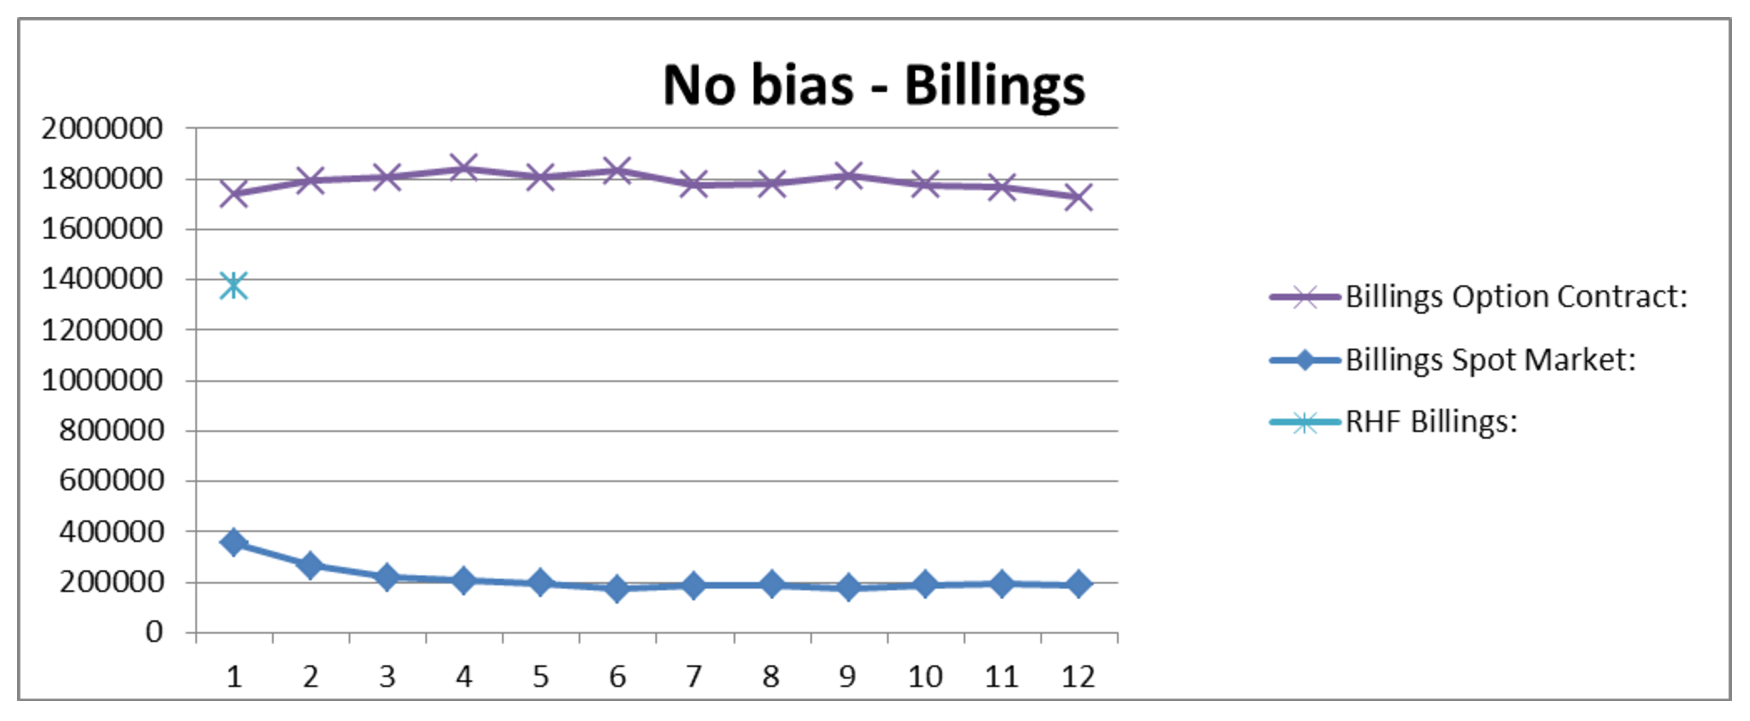
\includegraphics[width=.8\linewidth]{Figures/Unbiased_Option_Contract.eps}
  \caption{Unbiased DP}
  \label{fig:sfig1}
\end{subfigure}%
\begin{subfigure}{.5\textwidth}
  \centering
  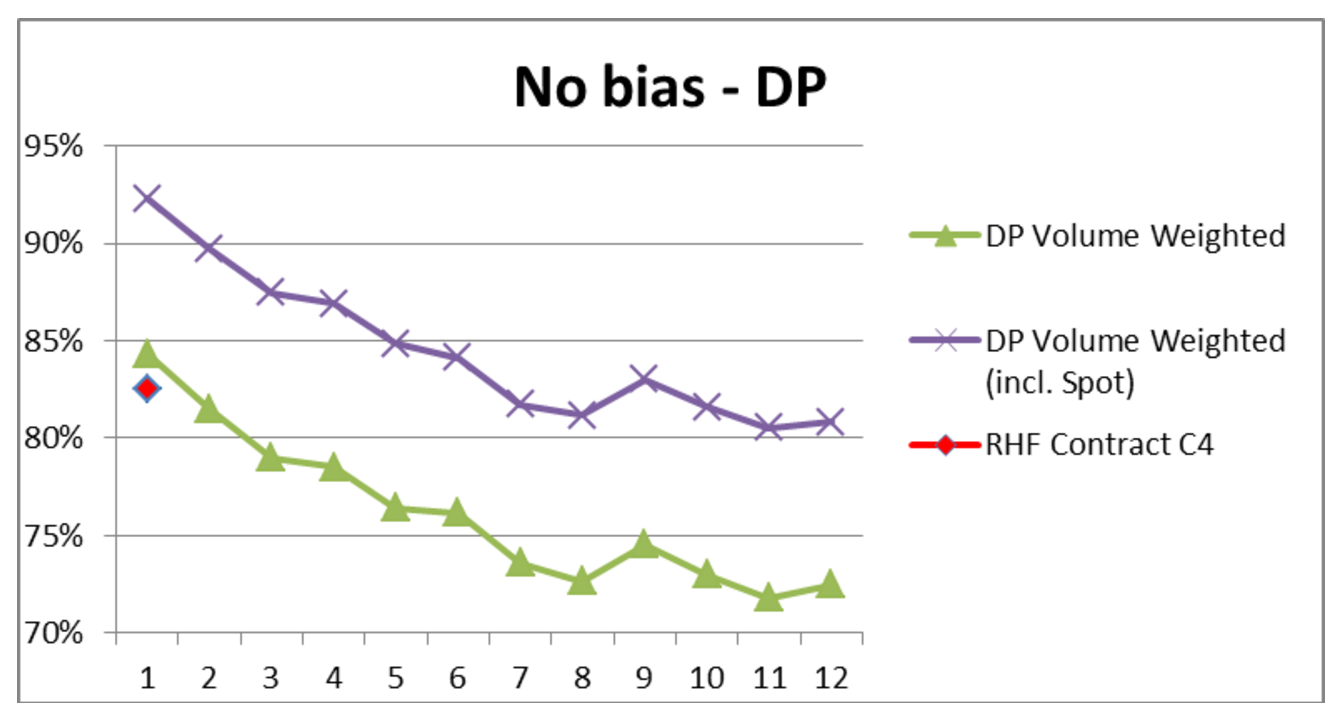
\includegraphics[width=.8\linewidth]{Figures/DP_Unbiased.eps}
  \caption{1b}
  \label{fig:sfig2}
\end{subfigure}
\caption{\label{fig:Overview-of-Option}Overview of Billings and Options within
 Capacity Reservation and Option Contract for Unbiased, Underplanning
 and Overplanning Customer order behavior}
\label{fig:fig}
\end{figure}

\begin{figure}
\begin{subfigure}{\textwidth}
  \centering
  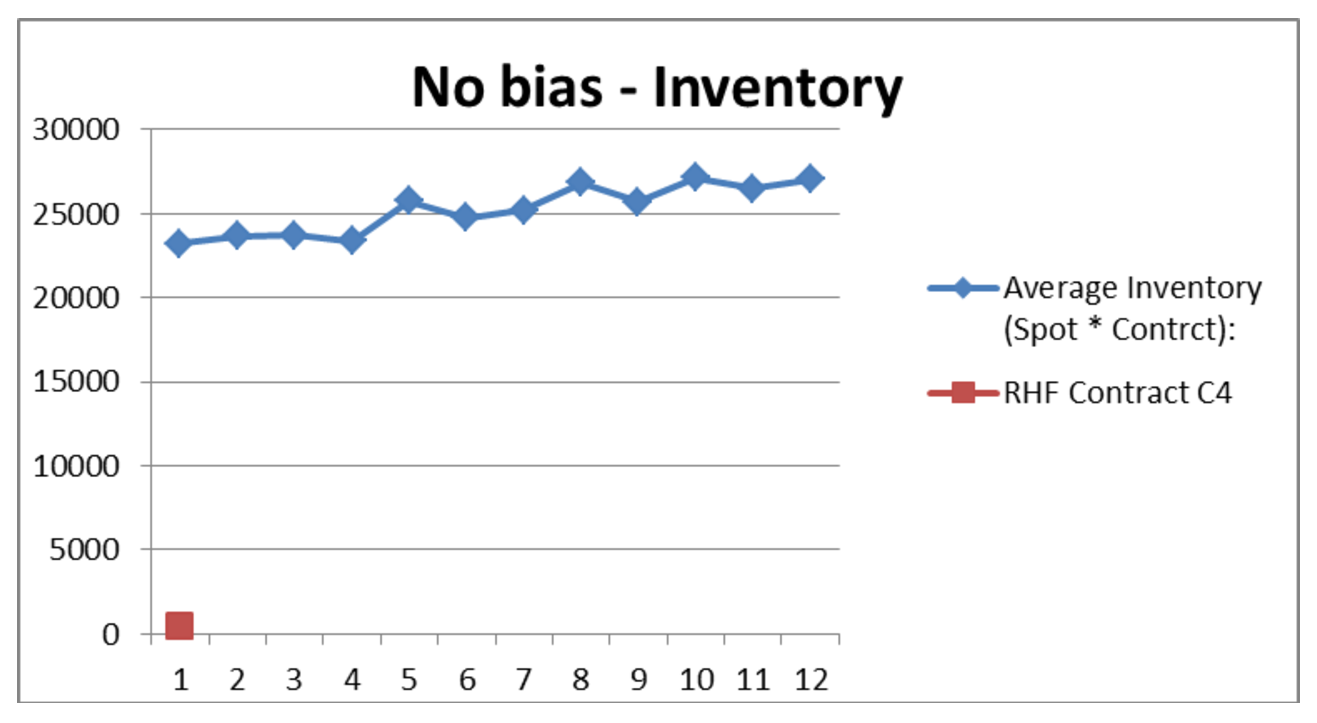
\includegraphics[width=0.75\textwidth]{Figures/Inventory_Unbiased.eps}
  \caption{Unbiased}
  \label{fig:sfig1}
\end{subfigure}%

\begin{subfigure}{\textwidth}
  \centering
  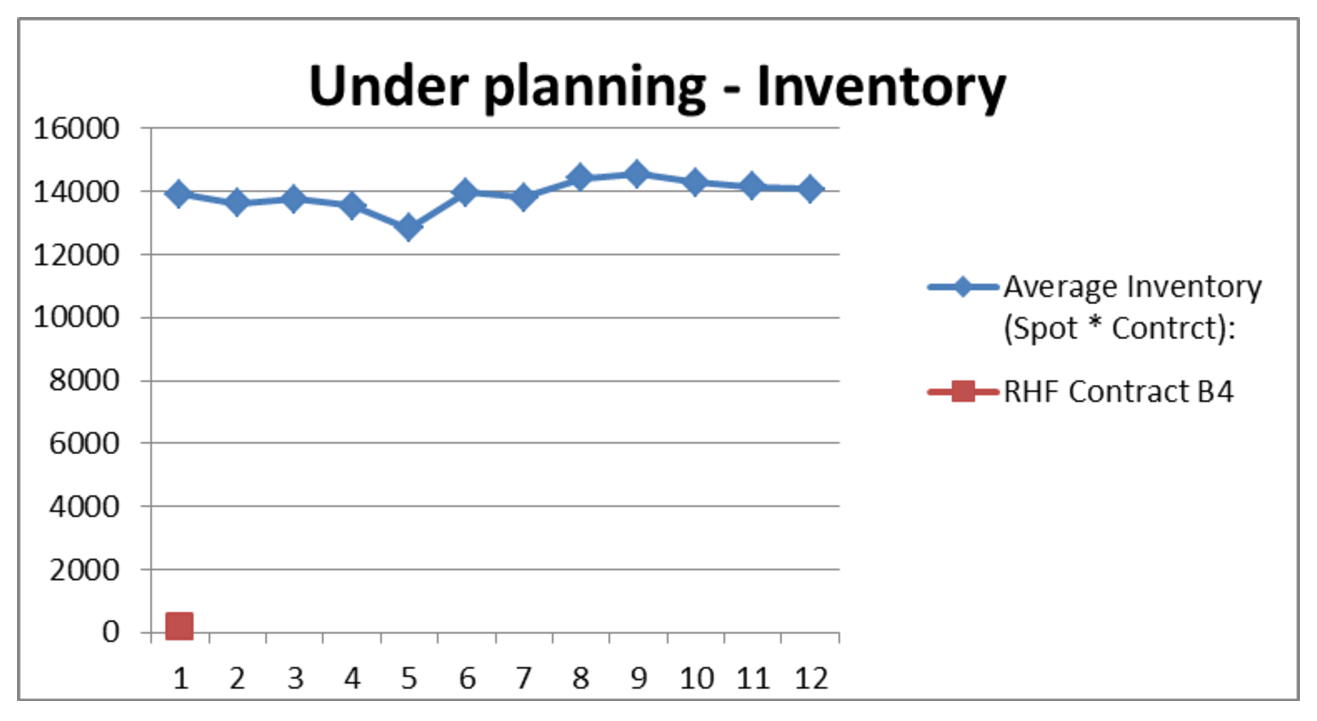
\includegraphics[width=0.75\textwidth]{Figures/Inventory_Underplanning.eps}
  \caption{Underplanning}
  \label{fig:sfig2}
\end{subfigure}

\begin{subfigure}{\textwidth}
  \centering
  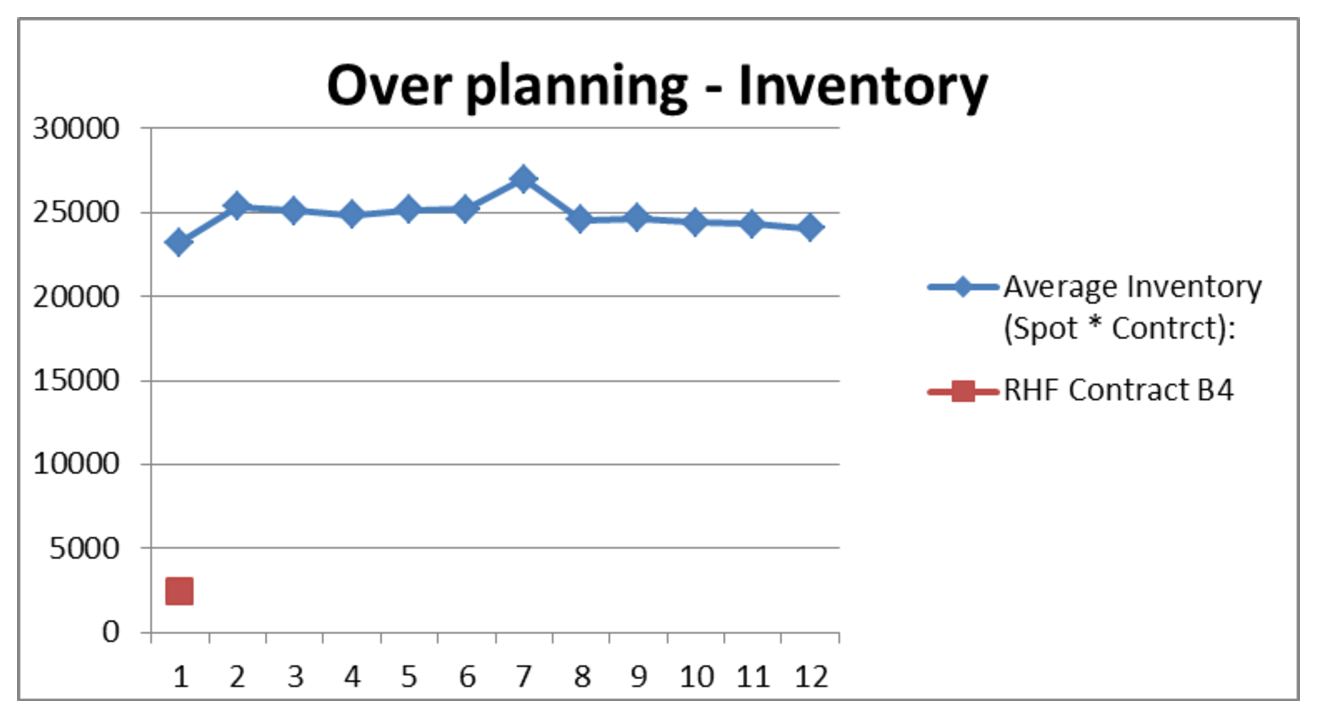
\includegraphics[width=0.75\textwidth]{Figures/Inventory_Overplanning.eps}
  \caption{Overplanning}
  \label{fig:sfig2}
\end{subfigure}
\caption{Overview of Billings and Options within
 Capacity Reservation and Option Contract for Unbiased, Underplanning
 and Overplanning Customer order behavior}
\label{fig:Overview-of-Option}
\end{figure}




 %\begin{figure}[h!]
 %\begin{center}
 %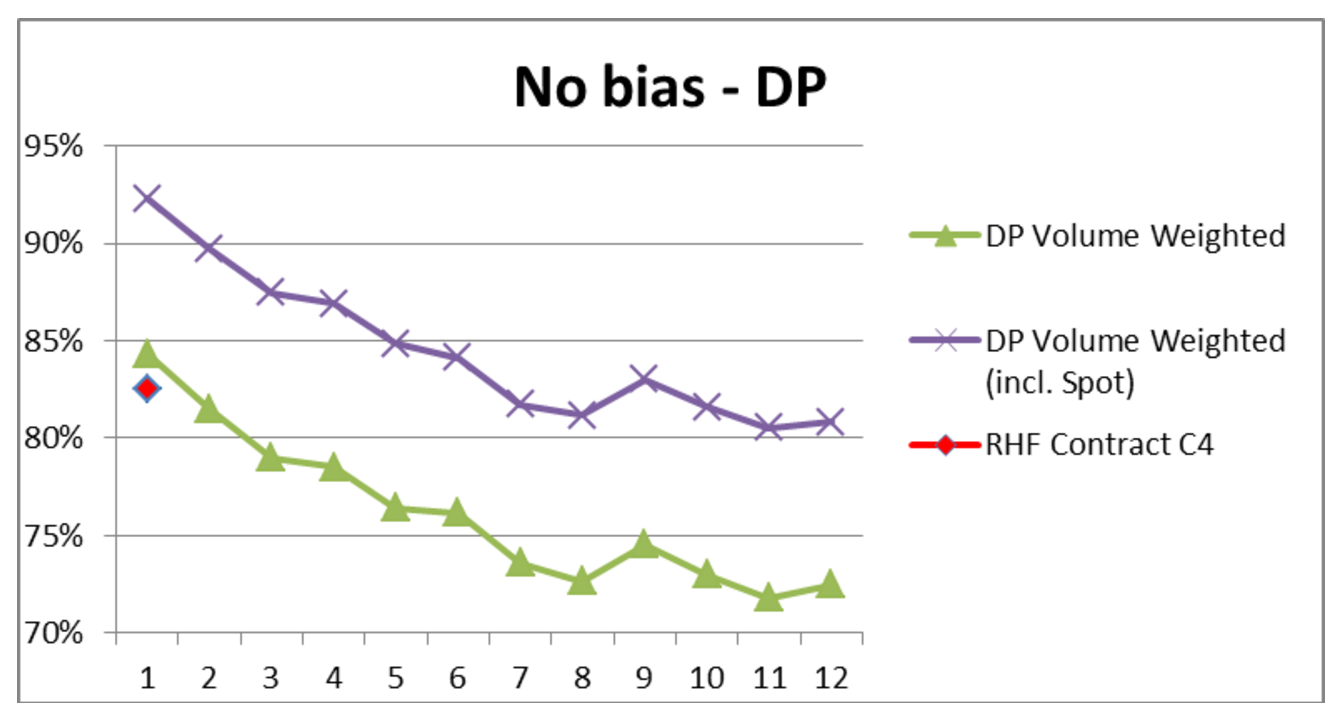
\includegraphics[width=0.5\textwidth]{Figures/DP_Unbiased.eps}
 %\caption{\label{fig:Overview-of-Option}Overview of Billings and Options within
 %Capacity Reservation and Option Contract for Unbiased, Underplanning
 %and Overplanning Customer order behavior}
 %\end{center}
 %\end{figure}

%\begin{figure}[h!]
% \begin{center}
% \includegraphics[width=0.7\columnwidth]{Figures/fig:Overview-of-Inventory.eps}
% \caption{\label{fig:Overview-of-Inventory}Overview of Inventory level with
% Capacity Reservation and Option Contract for Unbiased, Underplanning
% and Overplanning Customer order behavior}
% \end{center}
% \end{figure}

% \begin{table}
% \begin{tabular}{|c|c|c|c|c|c|c|c|}
% \hline 
% \multirow{2}{*}{No Bias} & Capacity Reservation Contract & \multicolumn{6}{c|}{Option Contract}\tabularnewline
% \cline{2-8} 
%  & No bias & 1 & 2 & 3 & 4 & 5 & 6\tabularnewline
% \hline 
% \hline 
% DP {[}\%{]} & 83 & 92  & 90  & 87  & 87  & 85  & 84 \tabularnewline
% \hline 
% Billings & 1374100 & 2274111  & 2348279  & 2147405  & 2135607  & 2124214  & 2136775 \tabularnewline
% \hline 
% Costs unused option fees &  & 59707 & 95669 & 40337 & 29084 & 41172 & 43177\tabularnewline
% \hline 
% Costs on spot market &  & 470056 & 353090  & 291395 & 271903 & 257763  & 229603\tabularnewline
% \hline 
% Inventory Costs & 14 & 696  & 710 & 712  & 701 & 773  & 743 \tabularnewline
% \hline 
% SC Profit & 1374086 & 1743651  & 1898811  & 1814961  & 1833918 & 1824507 & 1863253 \tabularnewline
% \hline 
% Profit compared to Capacity Reservation Contract {[}\%{]} &  & 21 & 28  & 24 & 25 & 25 & 26\tabularnewline
% \hline 
% \end{tabular}

% \begin{tabular}{|c|c|c|c|c|c|c|c|}
% \hline 
% \multirow{2}{*}{Under Planning} & Capacity Reservation Contract & \multicolumn{6}{c|}{Option Contract}\tabularnewline
% \cline{2-8} 
%  & Under Planning & 1 & 2 & 3 & 4 & 5 & 6\tabularnewline
% \hline 
% \hline 
% DP {[}\%{]} & 76  & 89  & 85  & 81  & 82  & 78  & 78 \tabularnewline
% \hline 
% Billings & 1374480  & 2582947  & 2575799 & 2594445 & 2565504 & 2547083  & 2561285\tabularnewline
% \hline 
% Costs unused option fees &  & 19480 & 19594  & 38015  & 19551  & 36078  & 36310\tabularnewline
% \hline 
% Costs on spot market &  & 404536  & 288815  & 255115 & 240157  & 224552 & 226029 \tabularnewline
% \hline 
% Inventory Costs & 6 & 418 & 409 & 413  & 407  & 385 & 419\tabularnewline
% \hline 
% SC Profit & 1374474 & 2158513  & 2266981  & 2300902 & 2305389 & 2286068 & 2298526\tabularnewline
% \hline 
% Profit compared to Capacity Reservation Contract {[}\%{]} &  & 36 & 39 & 40 & 40 & 40 & 40\tabularnewline
% \hline 
% \end{tabular}

% \begin{tabular}{|c|c|c|c|c|c|c|c|}
% \hline 
% \multirow{2}{*}{Over Planning} & Capacity Reservation Contract & \multicolumn{6}{c|}{Option Contract}\tabularnewline
% \cline{2-8} 
%  & Under Planning & 1 & 2 & 3 & 4 & 5 & 6\tabularnewline
% \hline 
% \hline 
% DP {[}\%{]} & 84 & 93 & 90 & 86 & 86 & 84 & 83\tabularnewline
% \hline 
% Billings  & 1373890 & 1595282 & 1595282 & 1586669 & 1594609 & 1564543 & 1577505\tabularnewline
% \hline 
% Costs unused option fees  &  & 38137 & 38211 & 45801 & 389808 & 46787 & 48087\tabularnewline
% \hline 
% Costs on spot market  &  & 366983 & 295295 & 244502 & 224978 & 207041 & 199415\tabularnewline
% \hline 
% Inventory Costs  & 75 & 696 & 761 & 753 & 745 & 755 & 756\tabularnewline
% \hline 
% SC Profit  & 1373815 & 118946 & 1261014 & 1295614 & 1329977 & 1309959 & 1329246\tabularnewline
% \hline 
% Profit compared to Capacity Reservation Contract {[}\%{]} &  & -6 & -9 & -6 & -3 & -5 & -3\tabularnewline
% \hline 
% \end{tabular}

% \protect\caption{\label{tab:Evaluation-of-Option}Evaluation of Option Contracts versus
% Capacity Reservation Contracts}

% \end{table}

% \section{Conclusion}

% This paper evaluated the use of Option Contracts in semiconductor
% supply chains, a market which experiences highly volatile demand due
% to exogenous demand with high forecast errors. Past work was reviewed
% on Option Contracts used in supply chains. Then a simulation model,
% consisting of one customer and one semiconductor manufacturer were
% presented to model a Capacity Reservation Contract typically used
% in semiconductor supply chains and Option Contracts. For the Option
% Contract, different delivery window lengths were analyzed with the
% used demand signal affected by a forecast error with differently biased
% customers (under planning, over planning, no bias). An evaluation
% of Option Contracts against Capacity Reservation Contracts was presented.
% These results show that the performance of the supply chain contracts
% heavily depends on the customer order behavior. For no Bias and under
% planning customer order behavior, the Option Contracts shows the potential
% to increase the overall profit of the supply chain by 21\% up to 40\%,
% whilst substantially improving supply chain service delivery, especially
% in the case that a spot market is set up. Whereas the capacity reservation
% contract seems more beneficial for customers with over planning behavior,
% as the customer has to pay a cancellation fee of
% 100\% in case he falls below the lower flexibility bound, whereas
% for the Option Contract the customer had to invest only the option
% price of 33\% of the product price. 



\bibliographystyle{plainnat}

\bibliography{KonstanzePaper2.bib}



\end{document}

